This section discusses how each database performed on implementing the kernels mentioned in Section \ref{sec:kernels} and discusses the effectiveness of each query language when producing a query to extract the required data for each kernel. 

The results of the data analysis can be viewed in Appendix \ref{app:analysis}.

\subsection{Priority 1 Mean Response Times}

\edt{JanusGraph can be seen to be far outperformed by the other two database technologies in terms of response times in Figure \ref{fig:sim1PerfResults}. This is a trend that features in all three queries regarding the medical response dataset. Another trend is that TigerGraph and PostgreSQL perform closely where TigerGraph responds the fastest.}

\edt{One observation is that it takes around 5 minutes for an ambulance to start from the time a call is made for a priority 1 emergency. This might be considered long for a life threatening situation but the personnel handling the call needs to carefully diagnose the situation before considering it priority 1 - so this is not unusual. There is more room to optimize the transfer times to hospitals by potentially adding another hospital to the area.}

\begin{figure*}[h]
    \centering
    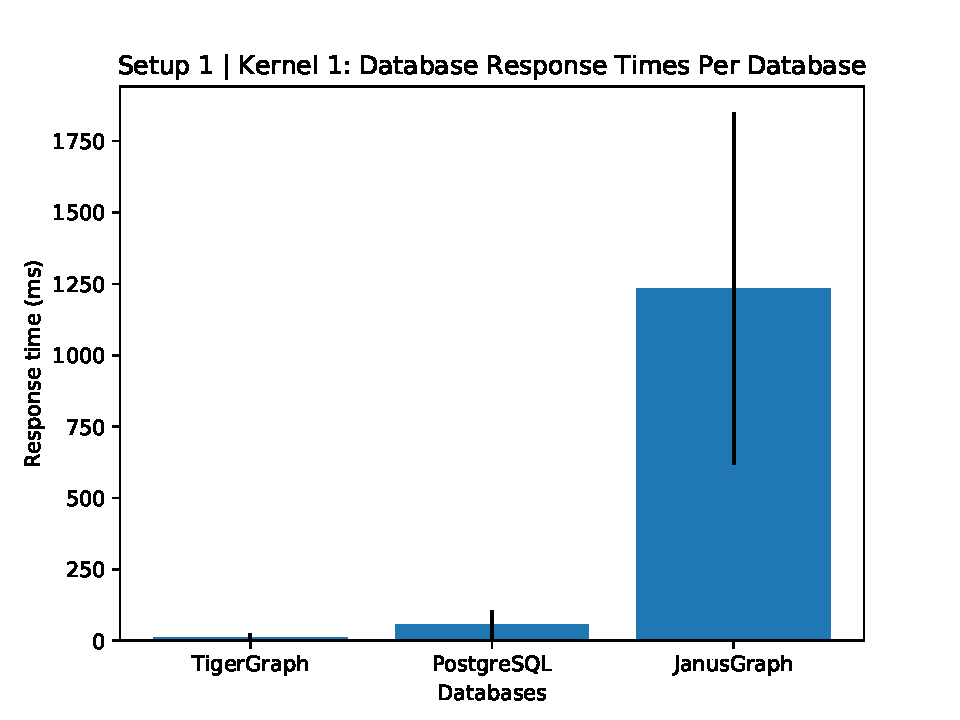
\includegraphics[width=0.49\textwidth]{img/7_simPerfResults/sim1PlotSetup1.pdf}
    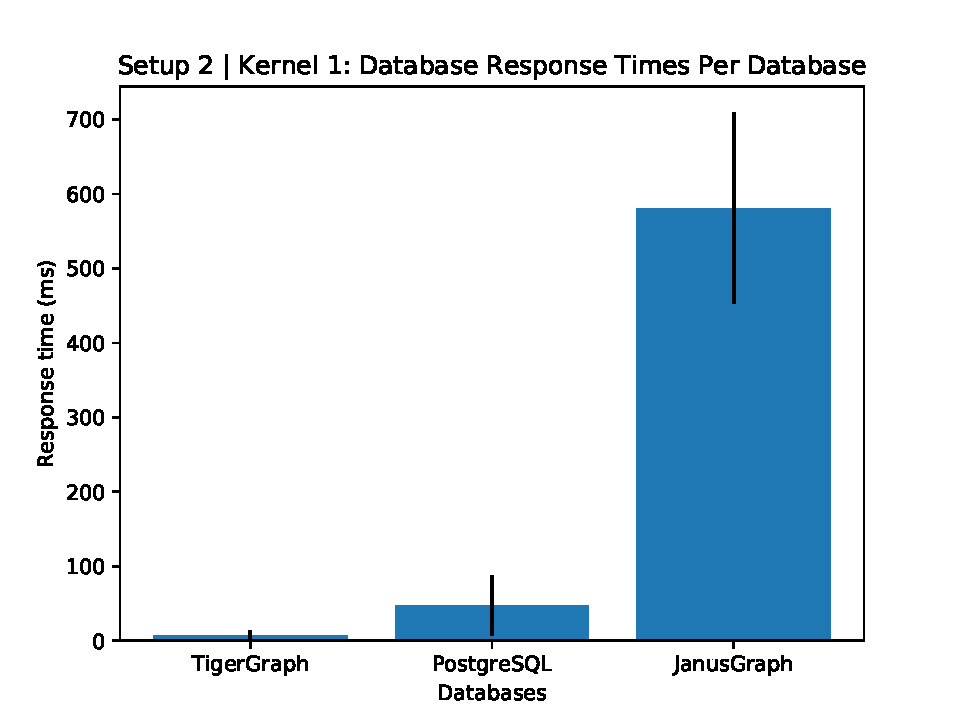
\includegraphics[width=0.49\textwidth]{img/7_simPerfResults/sim1PlotSetup2.pdf}
    \caption{Database response times using the medical response dataset for setup 1 and 2 for the kernel: ``Priority 1 Mean Response Times''. The error bars display standard deviation.}
    \label{fig:sim1PerfResults}
\end{figure*}


\subsection{Second Resource to Transfer Patients}

\edt{Each database appears to perform much more consistently (see Figure \ref{fig:sim2PerfResults}) with lower deviation as apposed to its performance in Figure \ref{fig:sim1PerfResults}. JanusGraph appears to have some kind of consistent overhead between the three containers (JanusGraph, Cassandra, and ElasticSearch) which appears to effect the response time.}

\edt{Regarding the result of this query (see Table \ref{tab:sim2Result}), it appears that more resources are sent to priority 2 emergencies. This simulation does not take into account emergencies that are recategorised on site which is something that happens outside of simulations. This could suggest that priority 2 responses are initially miscategorised and many should be priority 1 or that priority 2 responses simply require more resources in general.}

\begin{figure*}[h]
    \centering
    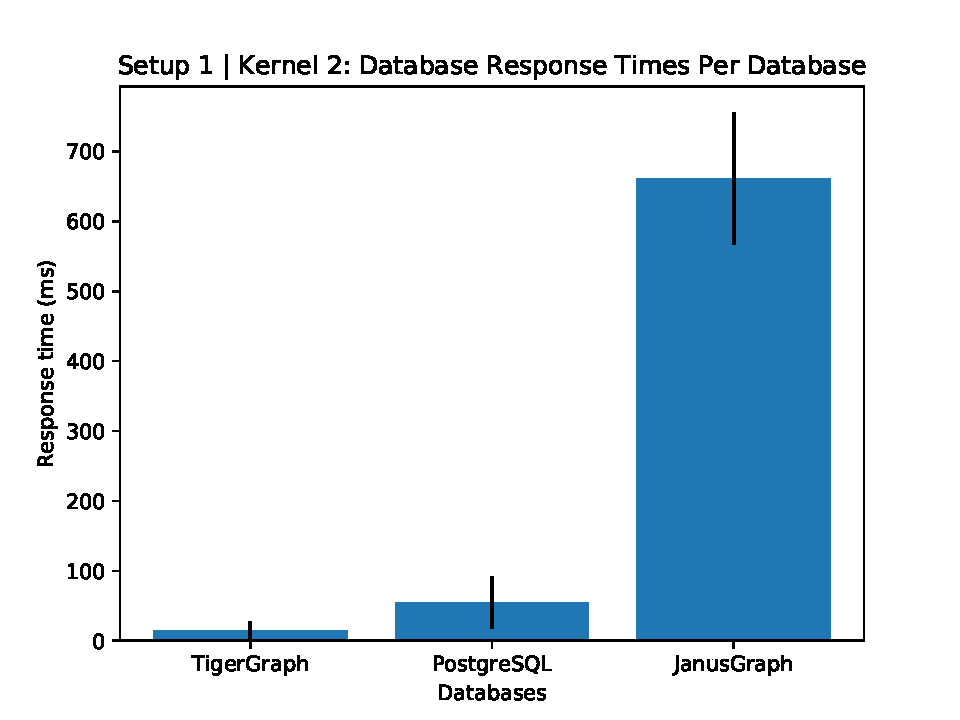
\includegraphics[width=0.49\textwidth]{img/7_simPerfResults/sim2PlotSetup1.pdf}
    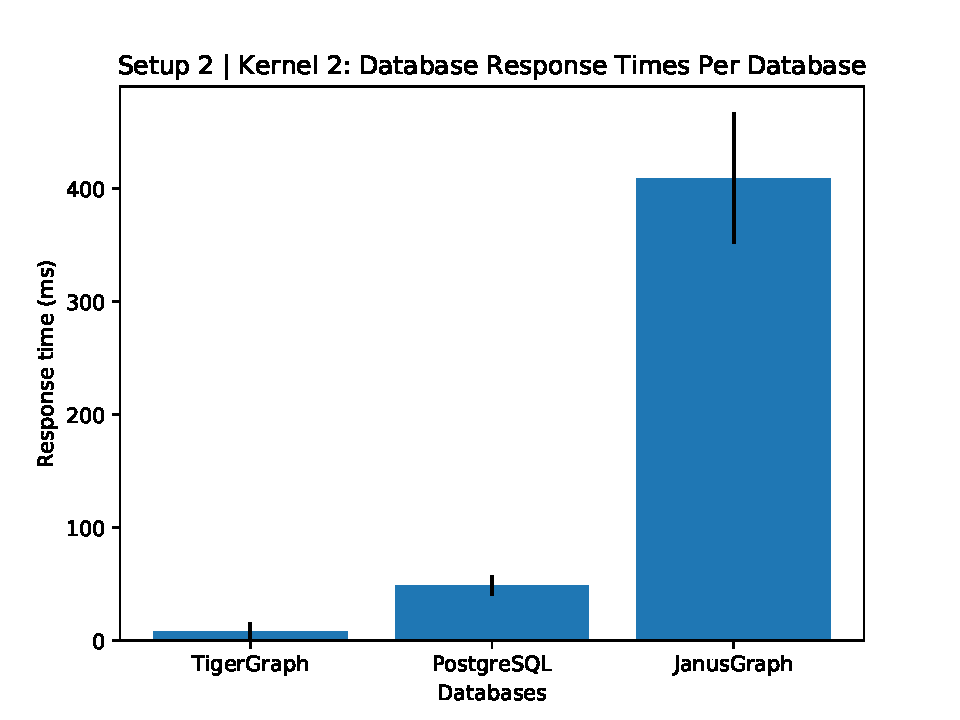
\includegraphics[width=0.49\textwidth]{img/7_simPerfResults/sim2PlotSetup2.pdf}
    \caption{Database response times using the medical response dataset for setup 1 and 2 for the kernel: ``Second Resource to Transfer Patients''. The error bars display standard deviation.}
    \label{fig:sim2PerfResults}
\end{figure*}

\subsection{Long Response Count}

\edt{This is only a temporal query and one can see that TigerGraph and PostgreSQL perform much more similarly than in the previous two queries. This suggests that added complexity from constraints in a query perform better in TigerGraph than in PostgreSQL.}

\edt{Although 15 minutes is considered quite fast for the whole response cycle to complete - which is why there are 5284 responses returned. This kind of query could be used to inform the medical infrastructure of a country or state how resource location affects response cycles.}

\begin{figure*}[h]
    \centering
    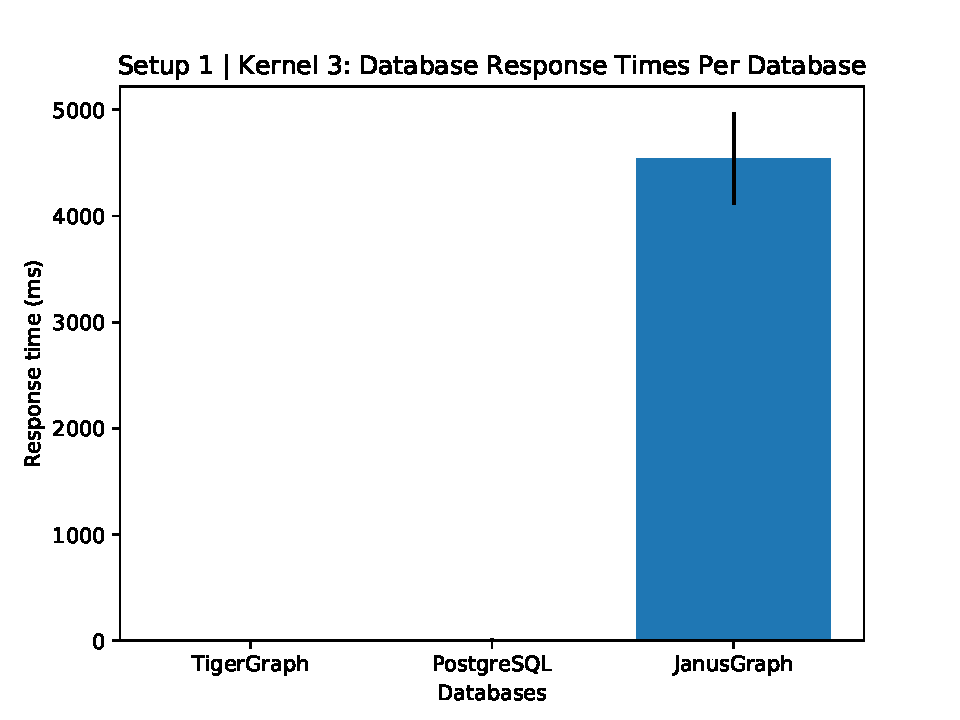
\includegraphics[width=0.49\textwidth]{img/7_simPerfResults/sim3PlotSetup1.pdf}
    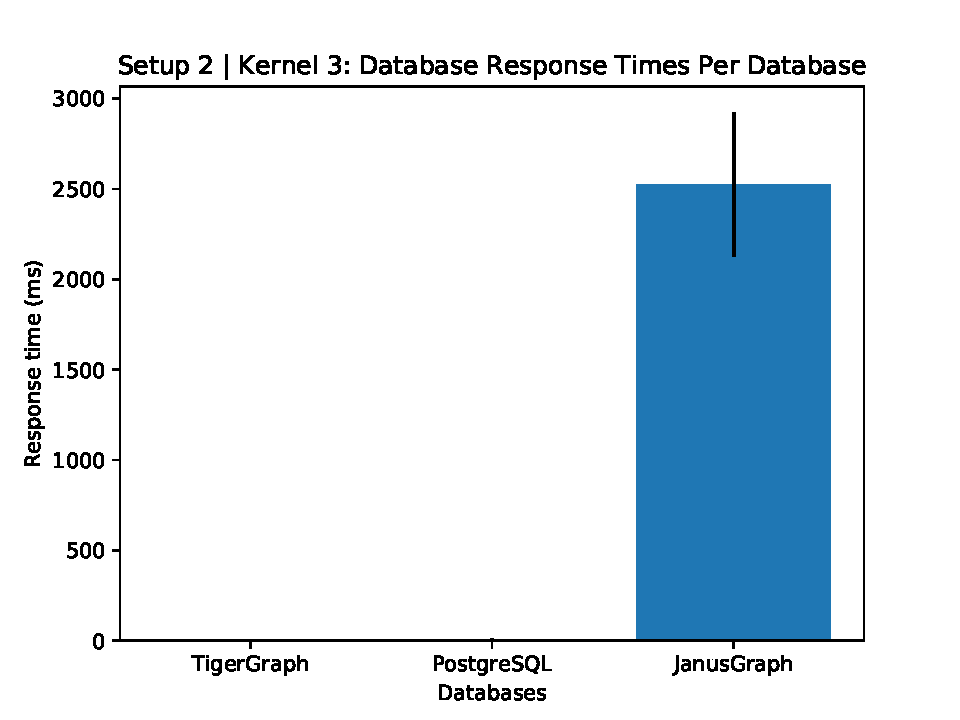
\includegraphics[width=0.49\textwidth]{img/7_simPerfResults/sim3PlotSetup2.pdf}
    \caption{Database response times using the medical response dataset for setup 1 and 2 for the kernel: ``Long Response Count''. The error bars display standard deviation.}
    \label{fig:sim3PerfResults}
\end{figure*}

\subsection{Kate's Restaurant Recommendation}

Figures \ref{fig:katePerfResults} shows linear growth in the response time of PostgreSQL whereas JanusGraph and TigerGraph remain fairly horizontal over increasing volumes of data. Due to the complexity of this query it comes as no surprise that the graph databases far outperform their relational counterpart. TigerGraph outperforms both PostgreSQL and JanusGraph in terms of query response time and shows a very high consistency as there is almost no standard deviation around the mean.

\begin{figure*}[h]
    \centering
    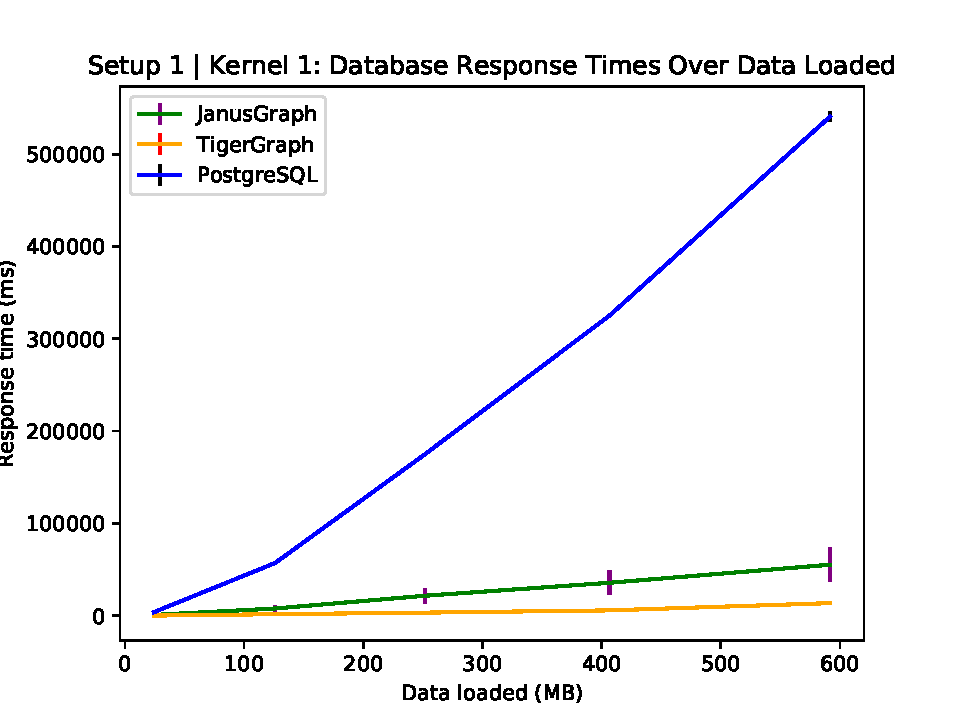
\includegraphics[width=0.49\textwidth]{img/7_yelpPerfResults/katePlotSetup1.pdf}
    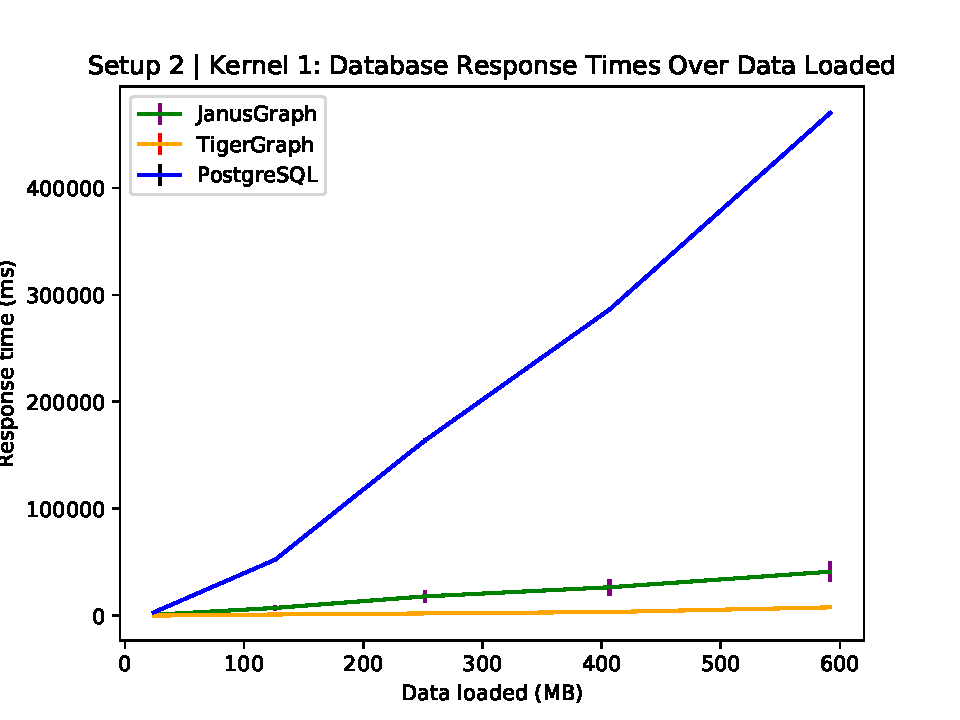
\includegraphics[width=0.49\textwidth]{img/7_yelpPerfResults/katePlotSetup2.pdf}
    \caption{Database response times over varying percentages of the Yelp dataset for setup 1 and 2 for the kernel: ``Kate's Restaurant Recommendation''. The error bars display standard deviation.}
    \label{fig:katePerfResults}
\end{figure*}

Table \ref{tab:kateResult} shows which restaurants would be recommended to Kate. One can see that both positive sentiment and star average over reviews for highly regarded restaurants compare well and remain consistent.

The reviews returned by the query were typically well above 3 stars and, since the Na\"ive Bayes performed well when predicting unseen text data, it comes as no surprise that most of the reviews were tagged as positive. Further analysis could look at how positive sentiment and star rating would compare for inconsistently performing restaurants, using a heuristic such as variance of mean star rating over time to indicate the consistency of restaurant performance. % but a special measure would need to be put in place to determine how ``inconsistency'' is measured.

\subsection{Review Trends in Phoenix 2018}
\label{sec:resultReviews2018}

Figure \ref{fig:reviewPerfResults} shows a phenomena of interest where JanusGraph performs poorly in relation to the other two database technologies with high deviation around the mean. PostgreSQL scales horizontally for this kernel which is most likely be due to the query being the simplest of the three kernels. TigerGraph outperforms both.

\begin{figure*}[h]
    \centering
    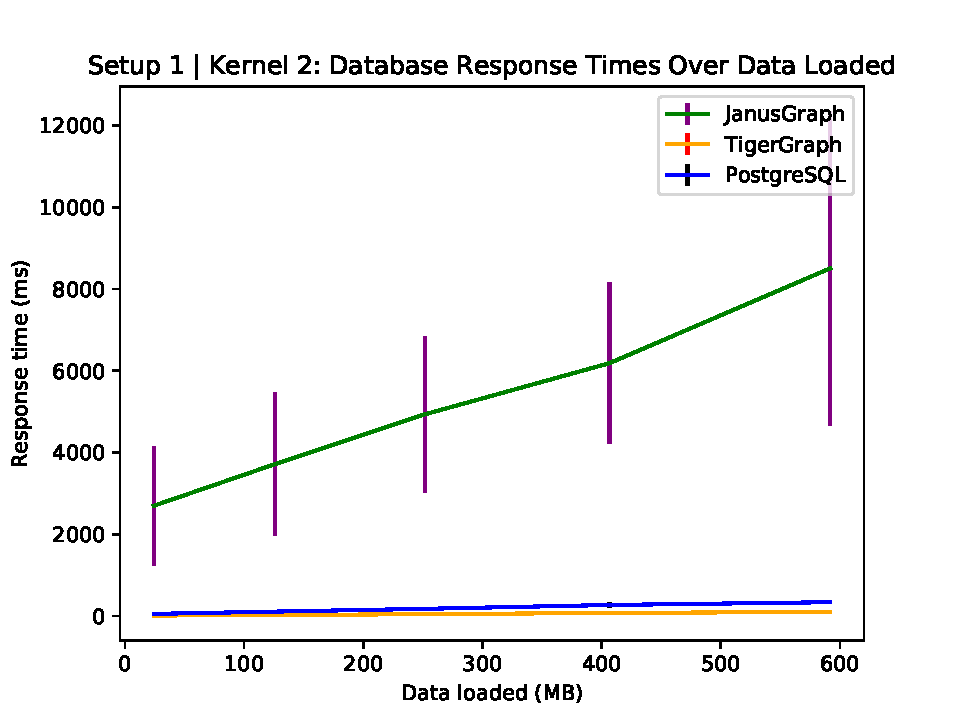
\includegraphics[width=0.49\textwidth]{img/7_yelpPerfResults/reviewsPlotSetup1.pdf}
    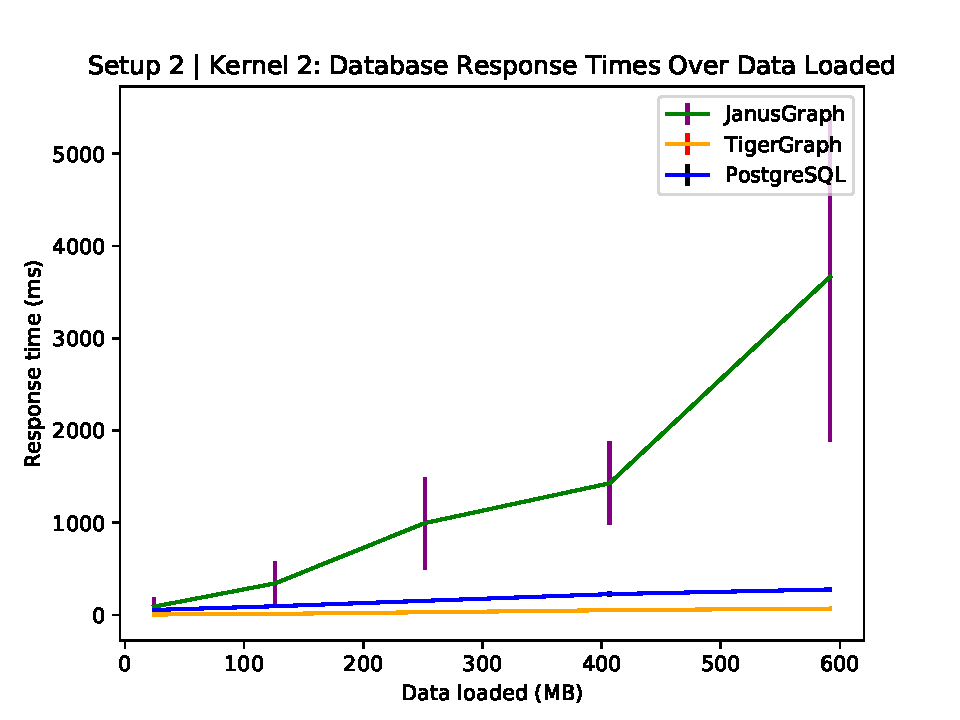
\includegraphics[width=0.49\textwidth]{img/7_yelpPerfResults/reviewsPlotSetup2.pdf}
    \caption{Database response times over varying percentages of the Yelp dataset for setup 1 and 2 for the kernel: ``Review Trends in Phoenix 2018''. The error bars display standard deviation.}
    \label{fig:reviewPerfResults}
\end{figure*}

The result of a subgraph produced by this query can be seen in Figure \ref{fig:reviewGraph}.

\begin{figure}[h]
    \centering
    \begin{mdframed}[backgroundcolor=gray!70!white, style=GraphFrame]
    {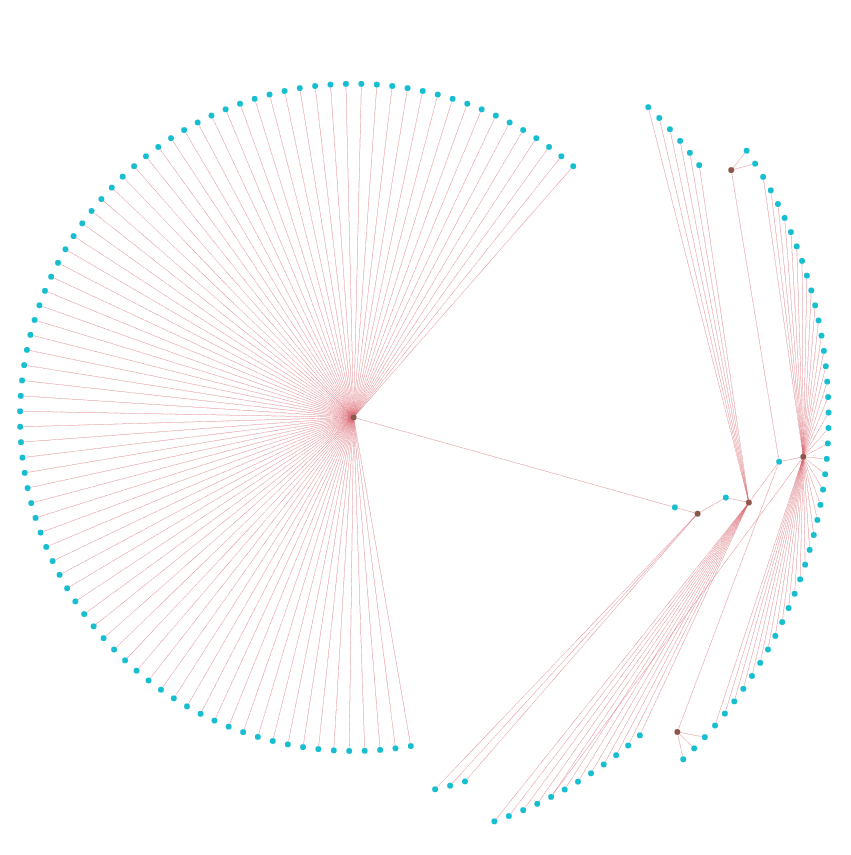
\includegraphics[width=\textwidth]{img/7_graphs/reviewsGraph.png}}
    \end{mdframed}
    \caption{A subset of the graph produced by TigerGraph on the result of the query for all reviews in the Phoenix area in 2018. Maroon edges represent reviews. Blue vertices are the users and brown vertices represent the businesses.}
    \label{fig:reviewGraph}
\end{figure}

The general trends shown in the review data for Phoenix during 2018 have the following characteristics:

\begin{itemize}
    \item More critical, lower scoring reviews tend to be longer and most useful.
    \item Reviews with 3 or 4 stars seem to be the funniest.
    \item Reviews with 4 or 5 stars tend to be the coolest.
\end{itemize}

The percentage positive sentiment, when scored relatively, is ordered consistently with the average star rating. This validates the performance of the binary sentiment classifier in that one almost does not need to see the star rating and can rely on text data alone when considering a broad spectrum of reviews.

This analysis could be performed over varied year brackets and different areas to see if performance is consistent or not. The implication of this could lead to experimenting with more sophisticated machine learning models on the dataset to be more precise in that it could potentially predict the star rating as is done in \cite{reddy2017prediction} and \cite{monett2016predicting}.

\subsection{Ranking Las Vegas by Friends' Sentiment}

Figure \ref{fig:cityPerfResults} shows both graph database technologies outperform PostgreSQL as PostgreSQL shows linearly growth as it did in Figures \ref{fig:katePerfResults}. For the experiments on 13\% of the dataset, JanusGraph shows a lot of deviation around the mean. This may be due to all the moving parts on which JanusGraph is implemented on and it's multi-level caching implementation behaving poorly at this size of the dataset.

\begin{figure*}[h]
    \centering
    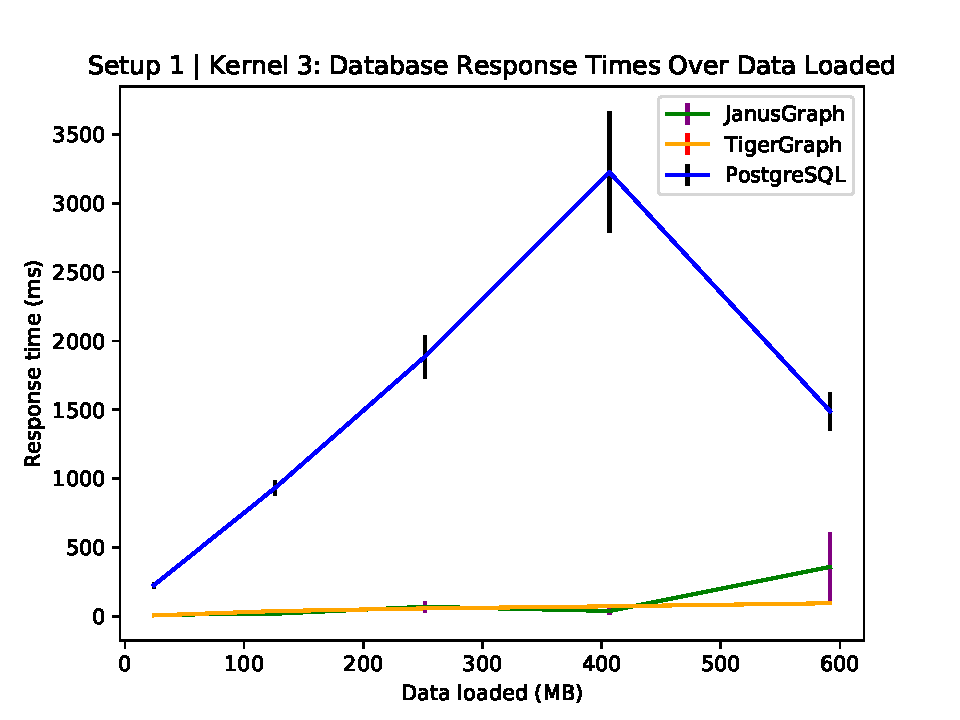
\includegraphics[width=0.49\textwidth]{img/7_yelpPerfResults/cityPlotSetup1.pdf}
    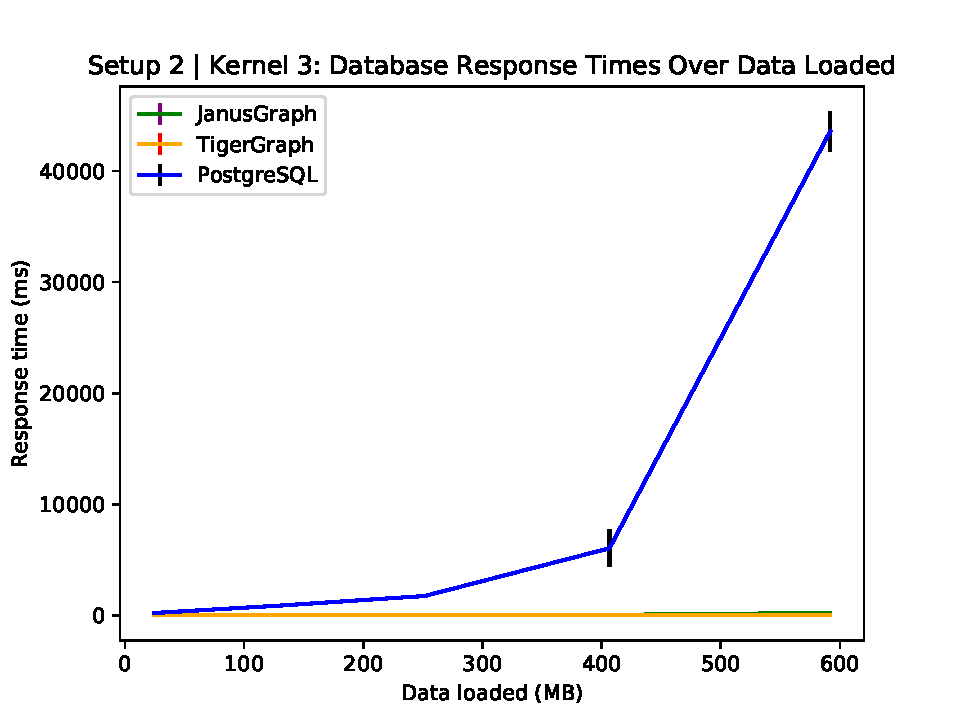
\includegraphics[width=0.49\textwidth]{img/7_yelpPerfResults/cityPlotSetup2.pdf}
    \caption{Database response times over varying percentages of the dataset for setup 1 and 2 for the kernel: ``Ranking Las Vegas by Friends' Sentiment''. The error bars display standard deviation.}
    \label{fig:cityPerfResults}
\end{figure*}

The result of this analysis was focused more on the performance rather than the data extracted. The results of the data analysis on this kernel does not show anything more interesting about the review data than what was already discussed in Section \ref{sec:resultReviews2018}. One notable difference in this kernel however, is that it produces a much more complex query and the databases perform accordingly.

This kernel shows that results may vary and can be correlated depending on the relationships between different data points.

\begin{figure*}[h]
    \centering
    \begin{mdframed}[backgroundcolor=gray!70!white, style=GraphFrame]
    {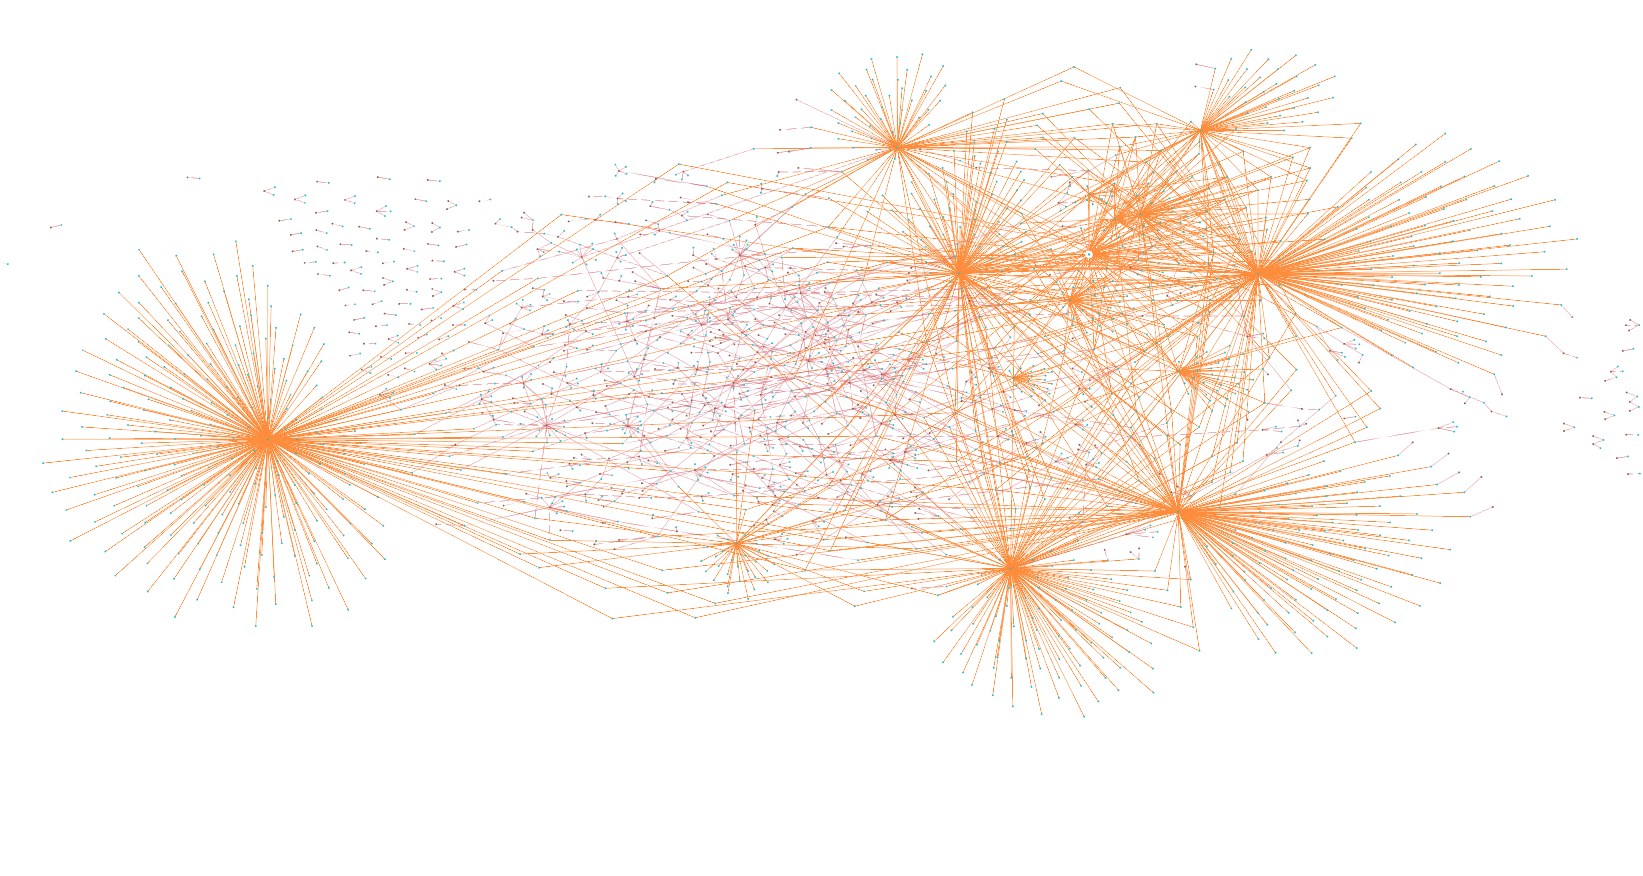
\includegraphics[width=\textwidth]{img/7_graphs/julieBusinesses.png}}
    \end{mdframed}
    \caption{A subset of the graph produced by TigerGraph on the result of the query for the third kernel, \emph{Ranking Las Vegas by Friends’ Sentiment}. Orange edges represent friend relations and maroon edges represent reviews. Blue vertices represent users and brown vertices represent businesses. The white center of the cluster on the top right is Julie and once can see the center of the giant cluster on the left is a mutual friend of Julie's. The topology of this graph suggests that Julie has direct and mutual friend circles whose influence extends well beyond her own.}
    \label{fig:cityGraph}
\end{figure*}

\begin{figure*}[h]
    \centering
    \begin{mdframed}[backgroundcolor=gray!70!white, style=GraphFrame]
    {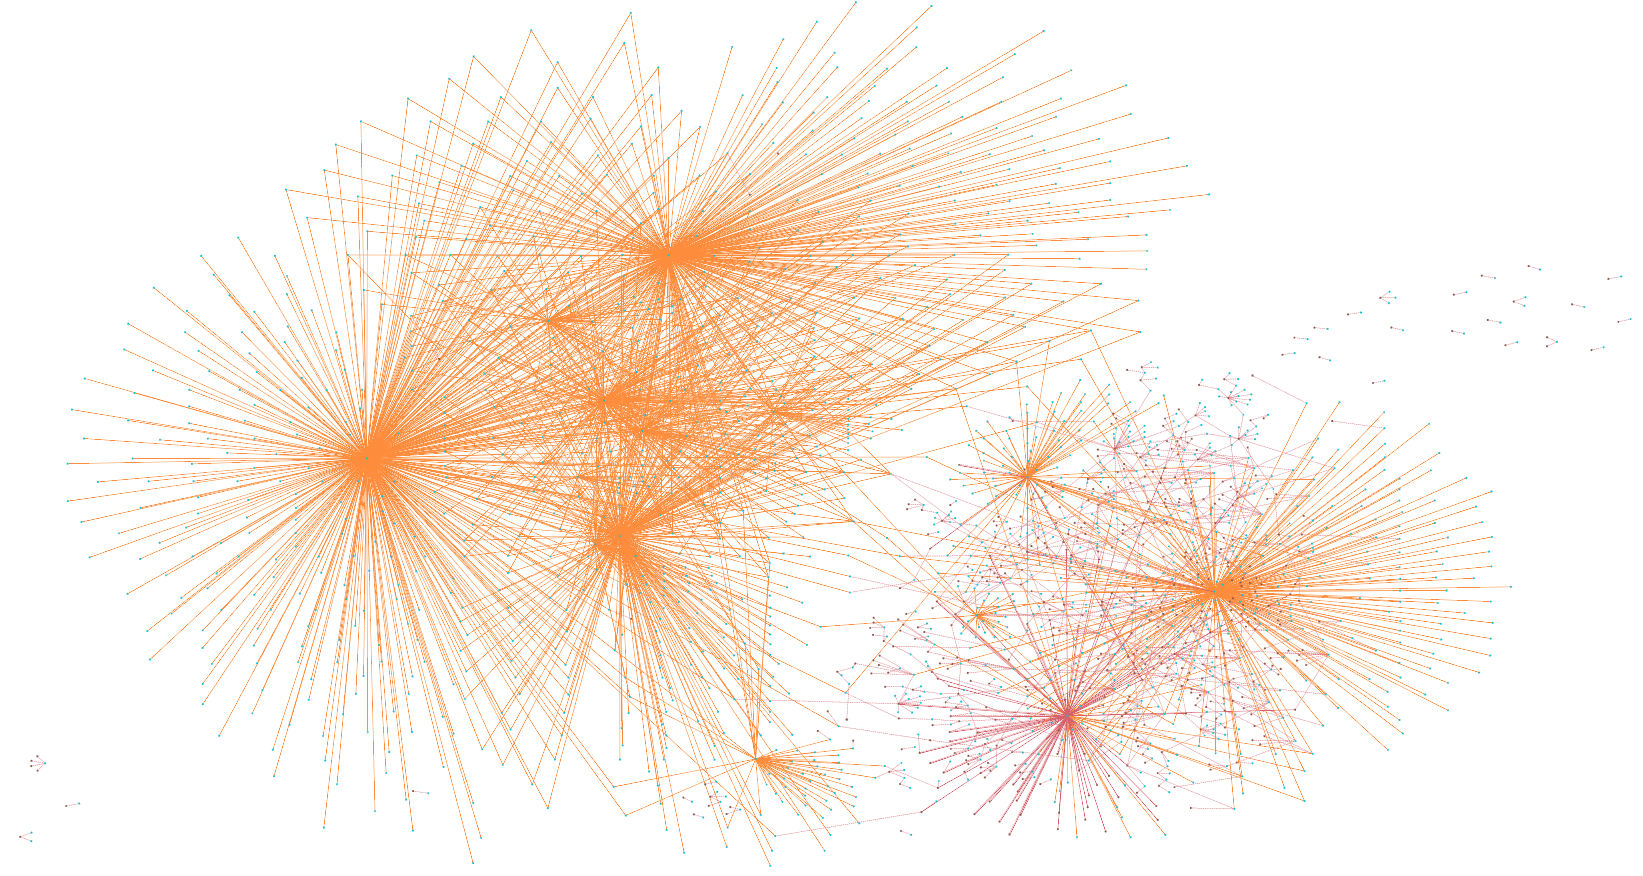
\includegraphics[width=\textwidth]{img/7_graphs/kateBusinesses.png}}
    \end{mdframed}
    \caption{A subset of the graph produced by TigerGraph on the result of the query for the third kernel, \emph{Ranking Las Vegas by Friends’ Sentiment} but on the user Kate from the first kernel. The topology of Kate's friend groups suggest a very cliquey circle of friends with influence not far from her own.}
    \label{fig:cityGraphKate}
\end{figure*}

\subsection{Memory Consumption}

\edt{The memory consumption of each database (while idle) is illustrated in Figure \ref{fig:memoryResults} and clearly shows the high cost of graph database technology with TigerGraph and JanusGraph using about 2GiB and 10GiB respectively. PostgreSQL only makes use of around 9MiB which makes is extremely lighter than the graph databases.}

\edt{The technologies used for JanusGraph all run on the JVM and, given the 32GB memory available, allowed the JVM's garbage collector to run infrequently. Most of the memory used by JanusGraph is in the cache for ElasticSearch, Cassandra, and JanusGraph, each storing an independent cache. Most of the fluctuations in memory came from the JanusGraph container and this happens from the moment the container is run. This cache can be limited by configurations but these results are from an unlimited cache setup as this is how the benchmarks were run.}

\edt{TigerGraph and PostgreSQL held constant (as their lower and upper memory bounds were within MiB differences) as the majority of those two databases are written in C or C++ which requires manual memory management. It is important to note that while JanusGraph uses a lot of memory, there are other graph database variants adhering to the Apache TinkerPop standard which claim to be more efficient in terms of memory such as Neo4j and OrientDB. Neo4j and OrientDB memory consumption is also configurable but may still use multiple GiB of memory because of the JVM \cite{neo4jMemory}\cite{orientDbMemory}.}

\begin{figure*}[h]
    \centering
    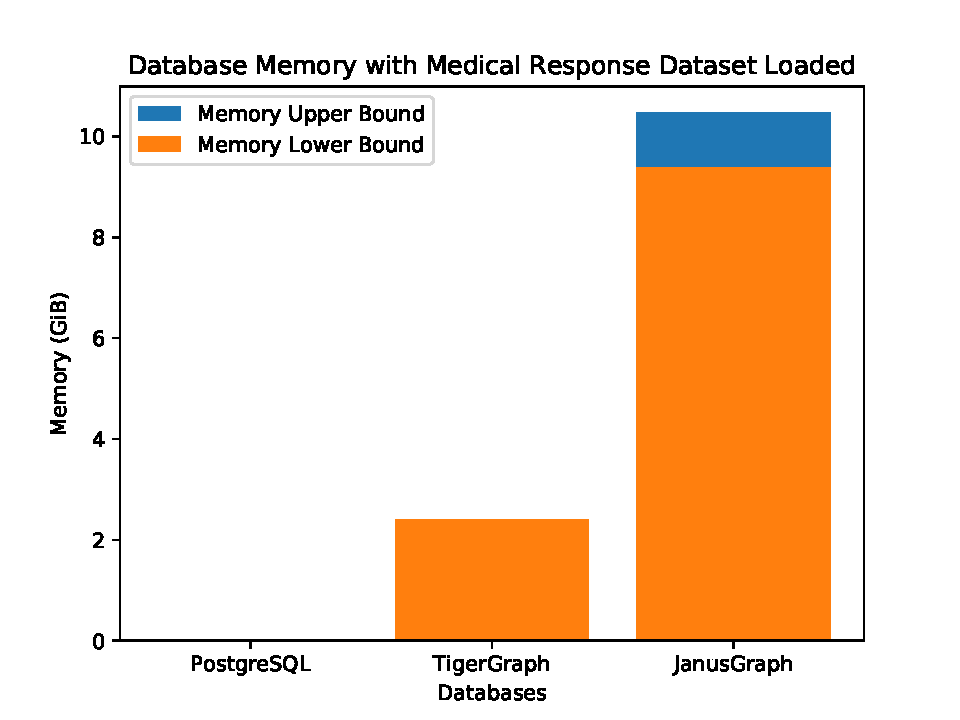
\includegraphics[width=0.49\textwidth]{img/7_memoryResults/simMemory.pdf}
    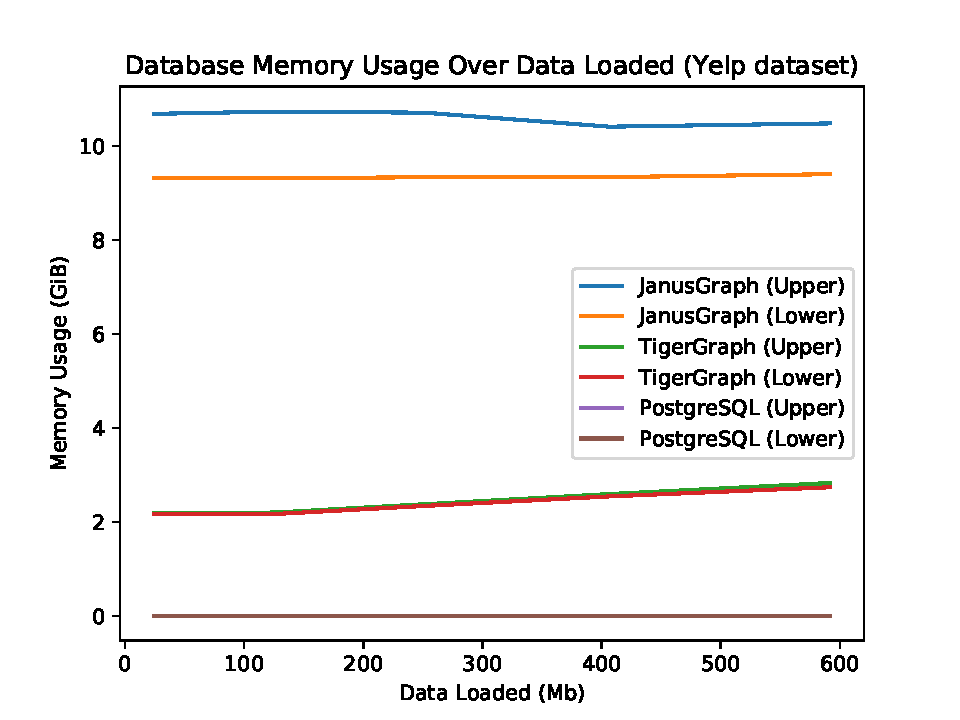
\includegraphics[width=0.49\textwidth]{img/7_memoryResults/yelpMemory.pdf}
    \caption{Database memory usage for each dataset. The medical response dataset is 1.5Mb large.}
    \label{fig:memoryResults}
\end{figure*}

\subsection{Queries}

\paragraph{SQL}

SQL is a mature and well supported querying language which makes it simple to implement a solution. The caveat to this simplicity is that the resulting solution may in complex cases lead to long and convoluted queries -- such as the one produced in Listing \ref{lst:sql1KateRestAppen}. The SQL queries produced for these kernels have a good balance between readability and expressiveness but, as complexity grew, so did size and queries began to lose the readability aspect.

SQL handles temporal data well and, in the PostgreSQL dialect, comes well supported with functions to operate on various temporal data types. This level of support provides ease of programming when implementing a SQL-based solution to a dataset with spatio-temporal properties.

\paragraph{Gremlin} 

Gremlin was found to produce the most concise queries of the three languages. The limitation of Gremlin is that, if one makes use of the mixed indexing search predicates, one may be limited to programming languages with support from these drivers to have the embedded Gremlin functionality. In the context of the technologies implemented in this investigation, a JVM language would be better suited as the back-end for a JanusGraph data storage solution. The Gremlin queries produced for these kernels were found to be readable in terms of describing the data flow of the traversal within a graph topology context. One may not enjoy Gremlin's referencing steps going back and forth within a query using the \texttt{as} and \texttt{select} steps but, after some experience with Gremlin, this will no longer be an issue.

The ability of certain steps allowing one to skip across edges to refer to vertices directly is part of why Gremlin is able to produce such concise queries. The performance of these queries heavily relies on the data flow produced by the ordering of such steps. This makes it important to use \texttt{filter} steps and be conscious of the ordering of each step.

Gremlin is well supported and has an extensive documentation\footnote{\url{http://tinkerpop.apache.org/docs/current/reference/}} but is a vastly different querying language when compared to SQL. The implication of this is that there is a small but significant learning curve involved. Effective imperative Gremlin queries will most likely only be written after some experience. Fortunately, Gremlin supports declarative querying which allows a user new to Gremlin to write effective queries with little experience.

\paragraph{GSQL} 

The GSQL queries produced by each kernel resulted in the queries with the most vertical space of the three query languages. This is necessary for segmentation of the query which is used for parallel graph traversals. The result of this segmentation and vertical space has made each query extremely readable and expressive. The conservative use of ASCII art and use of keywords from SQL provides a good balance between query visualization and familiarity. The development of queries using GraphStudio reduces the learning curve significantly as queries are developed in statically typed, compiler driven context -- only allowing one to install a query once all errors have been addressed. 

GSQL is well suited for spatial queries using the geo-grid approach -- which integrates well within a graph topology -- and temporal queries with a selection of built-in function for manipulating temporal data types -- as with SQL. By segmenting the query, the compiler is able to determine what can automatically be executed in parallel which adds to the fast response times of TigerGraph when compared to the other two databases.

The Rest++ API allows one to write a parameterized query once and access it anywhere without having to worry about driver issues other than being able to communicate with a REST API. This was a particular pleasure in the post-query development of connecting a web application back-end to communicate with TigerGraph.
